\chapter{Fundamentos}

Neste capítulo são estabelecidos os principais conceitos utilizados ao longo do projeto. Será feito uma breve abordagem sobre os fundamentos de serialização de dados; seguido pelo formato de representação JSON; o estilo de arquitetura baseado em recursos e, por fim, a ferramenta para consulta de dados sob demanda.

\section[Serialização de Dados]{Serialização de Dados}

Na ciência da computação, serialização de dados é um processo de tradução usado para converter estruturas de dados\footnote{
  Uma estrutura de dados é uma forma abstrata de representar e organizar dados. Seu objetivo é ajudar a reduzir complexidade, podendo armazenar dados de diferentes tipos, como números, strings ou até mesmo outras estruturas de dados.
} em formatos que possam ser armazenados, transmitidos e reconstruídos por um mesmo ou outro ambiente computacional. \cite{Cline2016}

Dados serializados normalmente vivem mais tempo que suas aplicações de origem e, ao ser armazenado em disco ou transmitido pela rede, são representados de modo diferente que sua estrutura em memória. Para se ler dados serializados em memória é preciso realizar o processo inverso, também chamado de deserialização, onde estes passam a ser representados por estruturas da linguagem de execução. \cite{Guller2016}

\begin{figure}[H]
  \centering
  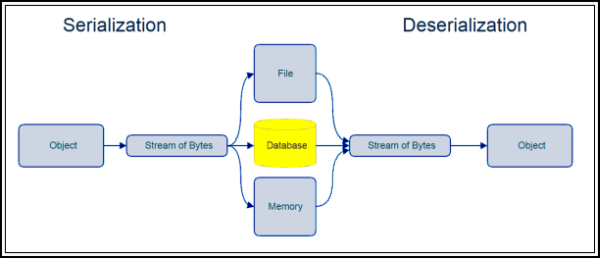
\includegraphics[width=\textwidth,height=\textheight,keepaspectratio]{figuras/data-serialization-deserialization.png}
  \caption{Processo de serialização e deserialização}
\end{figure}

Este processo, embora demande tempo, permitiu que aplicações fizessem o consumo de informações de forma distribuída, contribuindo com o aumento do volume de dados que circulam pela internet. Além disso, fez-se necessário a seleção adequada de formatos de serialização cuja estrutura não prejudique o desempenho de aplicações na busca por dados. \cite{SumarayMakki2012}

Segundo a Cisco Systems\footnote{
  Empresa de sistemas de rede.
}, no ano de 2015, houve um aumento de 21\% no volume de tráfego de dados registrados apenas por seus aparelhos. Sendo a categoria Web, Email e Data responsável por representar aproximadamente 7,558 petabytes de dados transmitidos por seus clientes durante um mês. \cite{Cisco2016}

Para suprir esta alta demanda, diversos formatos de serialização foram introduzidos para melhor atender os problemas de desempenho experienciados por serviços que disponibilizam dados serializados. Dentre eles, tempo de serialização e deserialização, tamanho de transferência, flexibilidade de uso, facilidade de leitura, automação, suporte para linguagem, entre outros. Contudo, cada formato possui seus prós e contras. \cite{Guller2016}

\begin{table}[ht!]
  \centering
  \resizebox{\columnwidth}{!}{
    \begin{tabular}{|c|c|c|c|c|}
      \hline
      Formato & Especificação & Codificação & Human-Readable & Esquema/IDL \\
      \hline
      XML & Padronizada & Textual & Sim & Sim \\
      JSON & Padronizada & Textual & Sim & Parcial \\
      YAML & Padronizada & Textual & Sim & Parcial \\
      Avro & Padronizada & Binário & Não & Sim \\
      Protocol Buffers & Padronizada & Binário & Parcial & Sim \\
      Thrift & Não Padronizada & Binário & Parcial & Sim \\
      \hline
    \end{tabular}
  }
  \caption{Comparação de formatos de serialização}
\end{table}

Para melhor entender o que define cada formato, será feito uma abordagem sobre as categorias de classificação usadas para estudar o comportamento dos formatos existentes hoje.

\subsection[Especificação]{Especificação}

Um formato pode ter sua especificação classificada como padronizada ou não padronizada. Uma especificação padronizada é regida por requisitos que auxiliam na reprodutibilidade do processo em outras linguagens para maximização da compatibilidade e minimização de erros. Ao contrário, dada uma linguagem de programação, não é garantido que sua implementação esteja seguindo os padrões e poderá ser considerado como não padronizada. \cite{McDermid1991}

\subsection[Codificação]{Codificação}

Codificação é o processo de sequenciamento de caracteres usado na redução da transmissão e armazenamento de dados. É possível classificar em dois tipos: textuais e binários. Formatos baseados em texto não são codificados para seu fácil acesso e podem ser lidos diretamente através de editores de texto. Já um formato binário faz o uso intensivo da codificação e decodificação para salvar espaço. \cite{Queiros2014}

\subsection[Human-Readable]{Human-Readable}

Ao representar estruturas de dados em formatos de serialização para que máquinas possam fazer a leitura, não é garantido, no entanto, que esta representação também seja legível por seres humanos.

Para que um formato seja human-readable, além de máquinas, pessoas devem conseguir ler e dizer o que está sendo representado mesmo fora de contexto. Para desenvolvedores, este detalhe é essencial no processo de debugging\footnote{
  Depuração é o processo de encontrar e reduzir defeitos num aplicativo de software ou mesmo em hardware.
}. Apesar do processo de serialização de dados não prever a ideia de escrita manual, se um formato é legível por pessoas então também é possível ser descrito por elas. Em geral, a maioria dos formatos baseados em texto são human-readable, enquanto os formatos binários não são. \cite{SumarayMakki2012}

Nota-se que a leitura de um formato é diferente de seu entendimento, uma vez que nem todos os formatos possuem maneiras de descrever seus metadados. Por exemplo, JSON é um formato baseado em texto e tem como objetivo a facilidade de uso e legibilidade por desenvolvedores. Contudo, nem sempre é possível identificar o que está sendo representado em suas estruturas. Através de extensões como JSON-LD e JSON Schema, é possível descrever meta informações para melhor entender o que está sendo representado sem perder a estrutura original do formato JSON.

\subsection[Esquema/IDL]{Esquema/IDL}

Com objetivo de entender o que está sendo representado, alguns formatos disponibilizam na sua especificação maneiras de descrever metadados. Esta categoria é importante principalmente para que máquinas consigam inferir quais estruturas estão sendo lidas e, assim, tomar decisões de forma autônoma.

Um formato descritivo normalmente disponibiliza estruturas como esquemas IDL\footnote{
  Linguagem de descrição utilizada para descrever a interface dos componentes de um software.
} para descrição da própria representação. À medida que estas descrições são incorporadas dentro da mesma representação, é possível classificar estes formatos como sendo auto-descritivos. \cite{Rentachintala2014}


\section{JSON}

JSON ou Javascript Object Notation é um formato de serialização de dados human-readable baseado em texto com especificação padronizada e parcialmente descritivo. Foi desenvolvido por Douglas Crockford com o objetivo de representar dados em uma maneira simples, leve e flexível através da redução na sobrecarga de marcações comparado ao formato XML.

Por ter se adaptado bem no ambiente de aplicações distribuídas, este formato acabou sendo amplamente utilizado em serviços como principal forma de representação de dados serializados. \cite{Duvander2013}

Na sua essência, o JSON foi construído com base em quatro tipos primitivos de dados e outros dois para composição. Cada tipo possui seu respectivo correspondente na maioria das linguagens de programação, embora possam ser identificados por nomes diferentes. \cite{Droettboom2015}

\begin{table}[H]
  \centering
  \begin{tabular}{|c|c|c|c|c|}
    \hline
    Tipo & Exemplo de Valor \\
    \hline
    object & \mintinline[fontsize=\small]{c}{ {"chave1": "valor1", "chave2": "valor2"} } \\
    \hline
    array & \mintinline[fontsize=\small]{c}{ ["primeiro", "segundo", "terceiro"] } \\
    \hline
    number & \mintinline[fontsize=\small]{c}{ 1, -1, 2.9999 } \\
    \hline
    string & \mintinline[fontsize=\small]{c}{ "Isso é uma string" } \\
    \hline
    boolean & \mintinline[fontsize=\small]{c}{ true, false } \\
    \hline
    null & \mintinline[fontsize=\small]{c}{ null } \\
    \hline
  \end{tabular}
  \caption{Tipos de valores em JSON}
\end{table}

Através da composição de listas, objetos e tipos primitivos, consegue-se representar complexas estruturas de dados. Não existe, no entanto, um único padrão de representação. Dada uma estrutura, é possível representá-la de inúmeras maneiras. A seguir estão duas formas diferentes de representação em JSON de uma entidade “pessoa”:
 \cite{Droettboom2015}

\begin{figure}[H]
  \centering
  \begin{minted}[frame=single,framesep=10pt,fontsize=\small]{javascript}
    {
      "nome": "Mateus Maso",
      "aniversario": "25 de março de 1992",
      "cidade": "Florianópolis, SC, Brasil"
    }
  \end{minted}
  \caption{Primeiro exemplo de representação JSON}
\end{figure}

\begin{figure}[H]
  \centering
  \begin{minted}[frame=single,framesep=10pt,fontsize=\small]{javascript}
    {
      "nome": "Mateus",
      "sobrenome": "Maso",
      "nascimento": "25-03-1992",
      "cidade": {
        "nome": "Florianópolis",
        "estado": "SC",
        "pais": "Brasil"
      }
    }
  \end{minted}
  \caption{Segundo exemplo de representação JSON}
\end{figure}

Ambas representações são válidas, apesar da figura 4 estar representando os dados em uma estrutura um pouco mais formal. No entanto, por ser um formato não descritivo, a responsabilidade de entender o que está sendo representado vai depender da análise crítica ou conhecimento prévio dos desenvolvedores. Já uma máquina, sem conhecer o contexto, não saberia como interpretar os dados de forma correta. \cite{Droettboom2015}

Para resolver isso, será abordado em seguida um dos formatos existentes hoje em dia para a descrição de estruturas JSON.

\section{REST}

REST ou Representational State Transfer é um estilo arquitetural usado para a comunicação de sistemas distribuídos através do protocolo HTTP. Foi introduzido por Roy Fielding em 2000 com o objetivo de oferecer às aplicações web um modelo de interface de acesso baseada em recursos. Além disso, descreve 6 tipos de restrições que serviços deveriam aplicar para ganho de performance, escalabilidade, simplicidade, modificabilidade, visibilidade, portabilidade e confiabilidade.

Vale lembrar que, por ter causado grande repercussão após sua publicação. O termo REST, segundo Richardson, acabou sofrendo diversas interpretações durante o tempo e, sua descrição representada de formas não originalmente propostas por Fielding. Alguns descrevem que serviços que violam essas restrições não podem ser considerados RESTful. Para Wildermuth, apesar de reconhecer as vantagens de cada restrição, serviços web devem usá-los de forma pragmatica. \cite{RichardsonEtAl2013} \cite{Wildermuth2015}

Apesar de ser introduzido num meio acadêmico, REST se adaptou bem em arquiteturas orientada a serviços. Segundo Pautasso, a eliminação da complexidade das soluções Web Services indicam que REST como uma solução aplicável para resolver problemas de integraçao de aplicaçoes empresariais e simplificar o encadeamento necessario para construir SOAs. A seguir, REST como adoção majoritária em relação a outros estilos para arquitetura de APIs. \cite{PautassoEtAl2008}

\begin{figure}[h]
  \centering
  \resizebox{\columnwidth}{!}{
    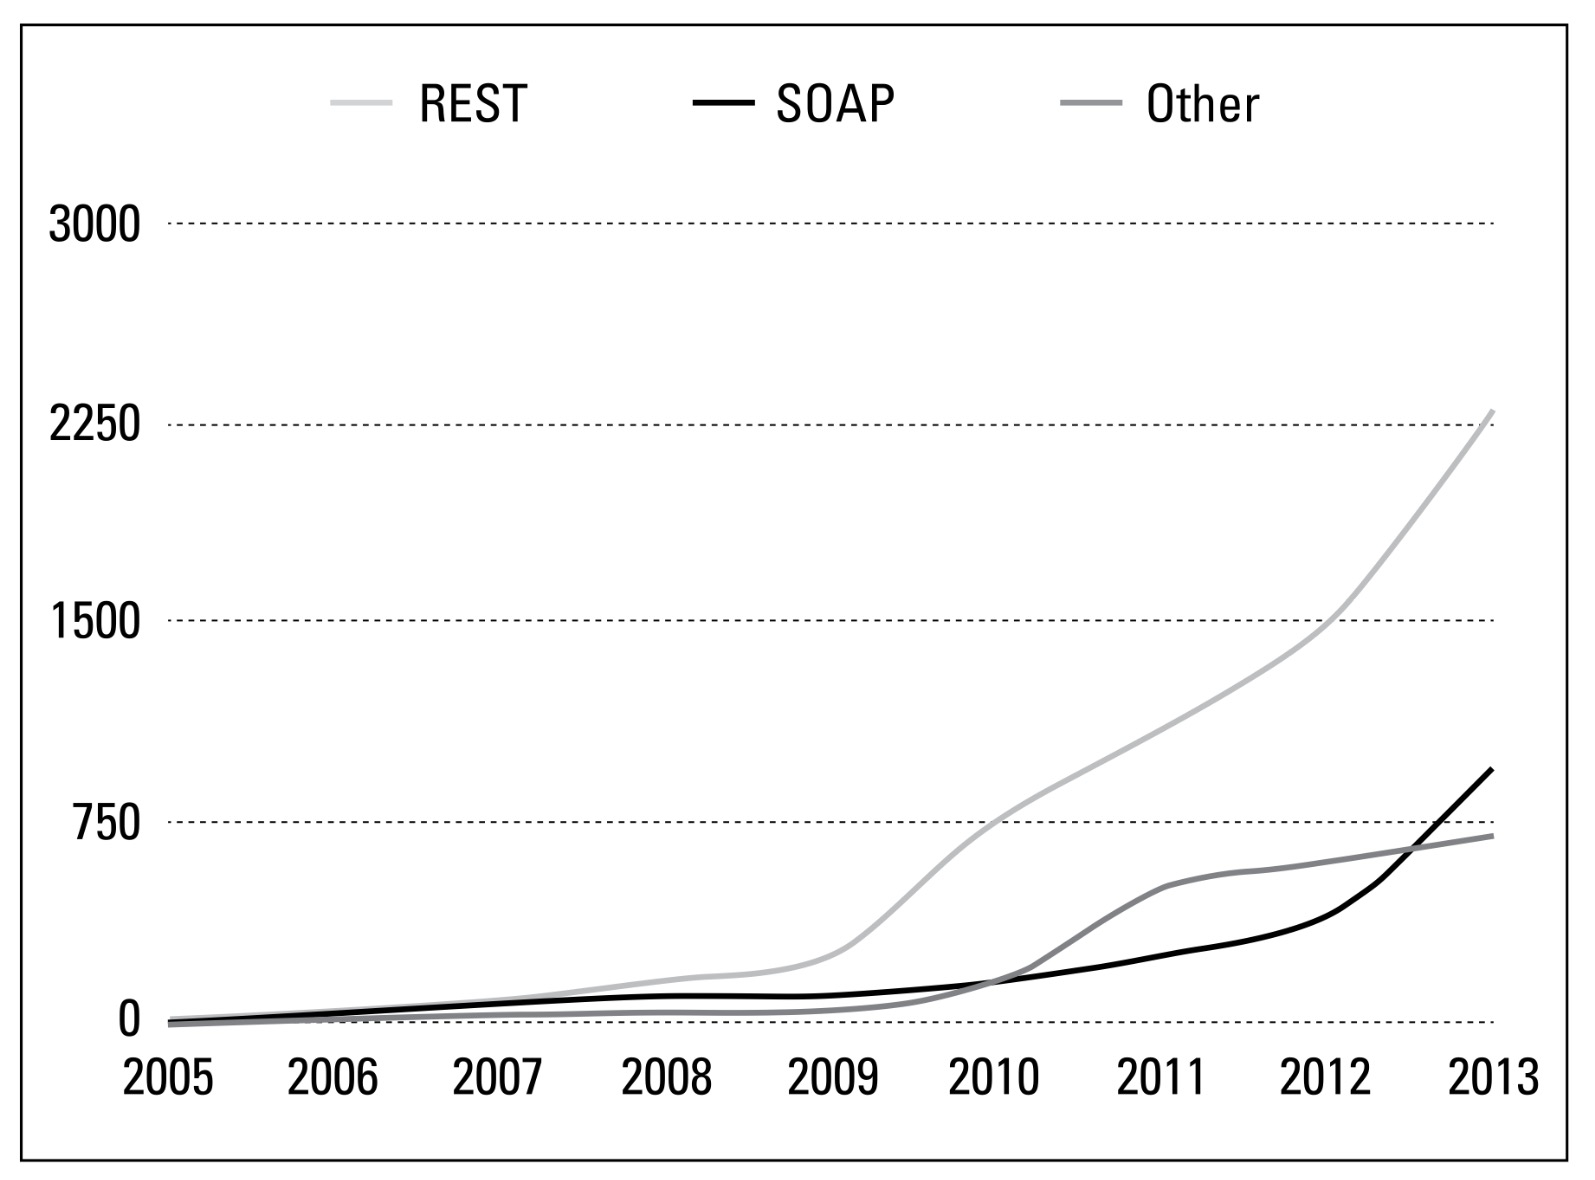
\includegraphics[width=\textwidth,height=\textheight,keepaspectratio]{figuras/api-styles.jpg}
  }
  \caption{Distribuição de estilos e protocolos para APIs}
\end{figure}

Sua maior vantagem de uso é por ser facilmente acessada por clientes web, mobile apps, dispositivos IoT. Isso permite que organizações construam clientes sem se preocupar com suporte à plataformas. Contudo, ao contrário de outros estilos de arquitetura, REST não sugere a criação de documentos de especificação, pois incentiva a escrita de respostas em hypertexo para navegação. Para Knupp, a idéia de documentação através de respostas autodescritivas dificulta a legibilidade, além de criar complexidade e informações adicionais. Ao invés, incentiva o uso de outras ferramentas de documentação e descrição de respostas. \cite{Knupp2016}

A seguir veremos sobre as restrições de arquitetura propostas pelo modelo REST, o que é uma API RESTful e seus níveis, além das atuais formas de documentação de APIs REST com suporte a leitura de máquinas.

\subsection[Restrições de Arquitetura]{Restrições de Arquitetura}

Esta seção fornece uma visão geral sobre as restrições propostas por Fielding para a implementação em arquiteturas web, além de ser examinado o impacto de cada restrição nesses sistemas distribuídos. \\

\textbf{Cliente-Servidor} \\

Nesta primeira restrição, não existe conexão entre cliente e servidor, mas sim a espera do servidor por pedidos de clientes através de chamada e resposta. O cliente (consumidor do serviço) não se preocupa com tarefas de comunicação de banco de dados, gerenciamento de cache, entre outros. Assim como o servidor (prestador de serviços) não está preocupado com as tarefas do cliente como interface ou experiência do usuário por exemplo. Permitindo a evolução independente dos dois ambientes, \textit{desde que sua interface de comunicação não seja alterada}. \cite{Fielding2000} \\

\textbf{Sem Estado} \\

Esta restrição ajuda na viabilidade, confiabilidade e escalabilidade de sistemas distribuídos, pois garantem que chamadas à API não estejam vinculadas a um determinado servidor. Como HTTP é um protocolo sem conexão, cada requisição deve conter todas as informações necessárias para que um servidor entenda o que um cliente está executando. Para Wildermuth, no entanto, dependendo da diversidade no número de clientes, ao manter um servidor sem estado, perder-se o controle no tamanho da estrutura de resposta necessária para atender a demanda de todos os clientes. \cite{Wildermuth2015} \\

\textbf{Interface Uniforme} \\

Em essência, Fielding propõe que aplicações façam o uso de verbos HTTP (POST, GET, PUT, DELETE) e identificadores uniforme de recursos (URI) para mapear operações em ambientes distribuidos e minimizar o acoplamento entre cliente-servidor. Essas regras de acesso são: \cite{Fielding2000}

\begin{itemize}[noitemsep]
\item Identificação de Recursos: Cada recurso deve ser disponibilizado através de uma URI específica e coesa. (Exemplo: GET /customers/1)
\item Manipulação de Recursos através de Representações: Um recurso pode ser representado em diferentes formatos para diferentes clientes. (Exemplo: HTML, XML, JSON)
\item Resposta Auto-explicativa: Metadados devem ser adicionados na requisição e resposta de um recurso para descrever seu estado atual ou desejado. (Exemplo: código de resposta HTTP, Host, Content-Type)
\item HATEAOS\footnote{
  Hypermedia as the Engine of Application State.
} - Caso um recurso possua relacionamentos, ao ser representado, estes devem estar especificados em forma de hiperlinks para facilitar a navegação de dados por clientes.
\end{itemize}

\textbf{Separação em Camadas} \\

Um dos princípios desta restrição está em evitar que clientes façam diretamente requisição para o servidor sem antes passar por um intermediário, como por exemplo um load balancer\footnote{
  Técnica para distribuir a carga de trabalho uniformemente entre dois ou mais computadores
}. Assegurando que clientes apenas se preocupem com a comunicação, deixando para que intermediários lidem com a distribuição de requisições. \cite{Fielding2000}

\begin{figure}[H]
  \centering  	   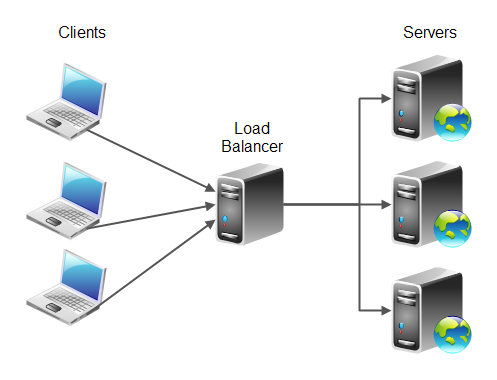
\includegraphics[width=0.7\textwidth,height=\textheight,keepaspectratio]{figuras/load-balancer.png}
  \caption{Exemplo de Load Balancer}
\end{figure}

\textbf{Código sob Demanda} \\

Apesar de ser a única restrição opcional do estilo, ela permite que servidores disponibilizem código em forma de script para que seja executado no cliente. Dessa forma, extendendo a lógica de serviço do servidor para seus clientes. \cite{Fielding2000} \\

\textbf{Cache} \\

Para aumentar desempenho de um serviço. Quando um recurso é acessado por mais de um cliente, se não houve mudança neste é recomendado que estas respostas sejam armazenadas em cache, evitando o processamento desnecessário. Isso significa que servidores, quando possível, devem implementar regras de cache para beneficio de ambos os ambientes. \cite{Fielding2000}

\subsection[RESTful]{RESTful}

Segundo Richardson, para que uma API de estilo REST seja consideirado RESTful, esta precisa seguir estritamente as regras exigidas anteriormente. Além disso, Richardson propõem uma escala de 4 níveis para avaliar a coesão e maturidade dessas APIs. \cite{RichardsonEtAl2013}

\begin{itemize}[noitemsep]
\item \textbf{Nível 0}: É a falta de qualquer regra; diz respeito ao uso de HTTP para operações de endereços no servidor. Normalmente, usa apenas um endpoint (URI) e um verbo HTTP.
\item \textbf{Nível 1}: Aplicação de recursos. A API é dividida em diferentes endpoints que indicam um ou mais recursos.
\item \textbf{Nível 2}: Implementação de verbos HTTP para diferentes tipos de operações. Onde uma mesma URI pode aceitar mais de um verbo para excução de diferentes procedimentos.
\item \textbf{Nível 3}: O conceito de HATEOS é aplicado para disponibilizar informações necessárias para interação e navegação da API.
\end{itemize}

\begin{figure}[H]
  \centering
  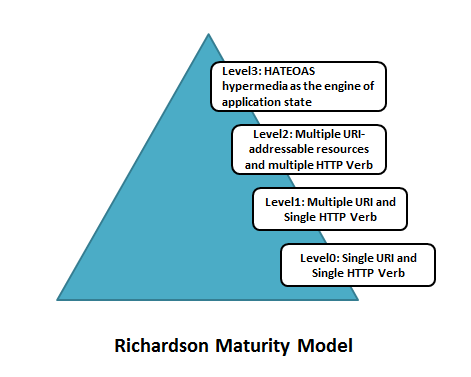
\includegraphics[width=0.8\textwidth,height=\textheight,keepaspectratio]{figuras/richardson-maturity-model.png}
  \caption{Modelo de Maturidade descrito por Richardson}
\end{figure}

\subsection[Descrições de API]{Descrições de API}

Em SaaS\footnote{
  Software as a Service.
}, APIs REST tornaram-se padrão como interface de acesso à serviços da empresa por seus clientes. A capacidade de oferer uma completa descrição sobre a api web para permitir que usuarios descubram e entam o serviço tornou-se critico para o sucesso da empresa. Contudo, apesar do processo de implementação tournou-se uma pratica comum, a definição de metadados de apis ainda não atingiu um grau de maturidade para normas amplamente aceitas. Apenas descrever manualmente APIs através de websites em linguagem natural permite que apenas pessoas entendam, isso se for bem projetada \cite{LuckyEtAl2016}

Com o fracasso de formatos tradicionais para descrição de web services como WADL, a adoção duvidosa de formatos hypermedia de resposta HATEOS como HAL e a demanda cada vez mais alta por boas especificações em formato legivel por humanos e maquinas. Nos últimos anos foram introduzidas diversas ferramentas e formatos de descrição para descrever Web APIs de REST, tanto em formatos legíveis para humanos como para máquinas. \cite{LuckyEtAl2016}

A seguir, comparações feitas por Sandoval entre as 3 linguagens mais usadas para especificação de APIs: \cite{Sandoval2015}

\begin{description}[leftmargin=8em,style=nextline]
  \item[\textbf{OpenAPI} (Swagger)] Pros: Amplamente adotada, grande comunidade, suporte pra diversas linguagens. \\ Cons: Carece de especificações de metadados mais avançadas.
  \item[\textbf{RAML}] Pros: Suporte a especificação avançada, adoção significativa, formato legível, bom suporte da indústria. \\ Cons: Falta de ferramentas de auxílio, não comprovada a longo prazo.
  \item[\textbf{API Blueprint}] Pros: Fácil de entender, simples de escrever \\ Cons: Pouca adoção, Carece de especificações de metadados mais avançadas, instalação complexa.
\end{description}

Recentemente, empresas como Heroku tem se dedicado ao uso do JSON Schema como formato de descrição de APIs, por ser uma tecnologia limpa e ainda pouco aplicada especificamente para a construção de grandes API \cite{Leach2014}. Já Lynn propõe um método de modelagem de REST API em serviços IoT utilizando JSON Hyper-Schema visto nos capítulos anteriores. Com suporte a descrição de entrada e saída de dados em toda a interface, junto com descrições URIs, relações e métodos que se aplicam aos links. Além disso, o formato suporta HATEOS e serve como entrada de documentação e ferramenta para geração de código. \cite{LynnEtAl2016}


\section{GraphQL}

GraphQL é uma linguagem de consulta de dados e interpretador para APIs. Foi desenvolvida pela Facebook em 2012 mas sua especificação apenas publicada em 2015. Tem com objetivo fornecer uma descrição completa e compreensível dos dados disponíveis em APIs. Além disso, dá aos clientes o poder de trabalhar apenas com as estrutura de dados que precisam, torna mais fácil evoluir APIs ao longo do tempo e permite o desenvolvimento de ferramentas em cima de sua linguagem. \cite{GraphQL2016}

Importante ressaltar que GraphQL não está preso a algum banco de dados especifico ou mecanismo de armazenamento. Ao invés, é utilizado para consultar código já existente ou estruturas de dados. Para criar um esquema, é preciso definir os tipos de estruturas, seus campos de acesso e funções para mapear e retornar dados reais em código. \cite{GraphQL2016}

Por ser uma especificação, GraphQL possui implementações em diversas linguagens de programação e atualmente é usado em diversos contextos, sendo eles para comunicação entre cliente-servidor, microserviços, simplificação de APIs, navegação de árvores, gerador de consultas para banco de dados, entre outros.

\begin{figure}[h]
  \centering
  \inputminted[frame=single,framesep=10pt]{javascript}{anexos/graphql-schema.gql}
  \caption{Esquema GraphQL}
\end{figure}

\begin{figure}[h]
  \centering
  \inputminted[frame=single,framesep=10pt]{javascript}{anexos/graphql-code.js}
  \caption{API de um código em JavaScript}
\end{figure}

Uma vez que um serviço GraphQL está sendo executado (normalmente a uma URL em um serviço web), pode ser enviado consultas GraphQL para validar e executar. Uma consulta recebida é primeiro verificado para garantir que ele só se refere aos tipos e campos definidos, em seguida, executa as funções fornecidas para produzir um resultado. \cite{GraphQL2016}

\begin{figure}[h]
  \centering
  \inputminted[frame=single,framesep=10pt]{javascript}{anexos/graphql-query.gql}
  \caption{Query GraphQL para esquema}
\end{figure}

\begin{figure}[h]
  \centering
  \inputminted[frame=single,framesep=10pt]{javascript}{anexos/graphql-query-response.json}
  \caption{Resposta JSON da Query GraphQL}
\end{figure}

\subsection[Linguagem de Consulta]{Linguagem de Consulta}

Clientes que buscam realizar consultas de dados em serviços GraphQL precisam antes entender seu formato de requisição, também chamado de documento. Um documento contém operações como consultas e mutações. Além disso, é possível especificar fragmentos, uma unidade comum de composição para reuso de consultas. \cite{GraphQL2016}

\textbf{Sintaxe}

A GraphQL query document describes a complete file or request string received by a GraphQL service. A document contains multiple definitions of Operations and Fragments. GraphQL query documents are only executable by a server if they contain an operation. If a document contains only one operation, that operation may be unnamed or represented in the shorthand form, which omits both the query keyword and operation name. Otherwise, if a GraphQL query document contains multiple operations, each operation must be named.

There are two types of operations that GraphQL models: query a read-only fetch. mutation, a write followed by a fetch. Each operation is represented by an optional operation name and a selection set. If a document contains only one query operation, and that query defines no variables and contains no directives, that operation may be represented in a short-hand form which omits the query keyword and query name. An operation selects the set of information it needs, and will receive exactly that information and nothing more, avoiding over-fetching and under-fetching data. In this query, the id, firstName, and lastName fields form a selection set. Selection sets may also contain fragment references.

A selection set is primarily composed of fields. A field describes one discrete piece of information available to request within a selection set. Some fields describe complex data or relationships to other data. In order to further explore this data, a field may itself contain a selection set, allowing for deeply nested requests. All GraphQL operations must specify their selections down to fields which return scalar values to ensure an unambiguously shaped response. Fields are conceptually functions which return values, and occasionally accept arguments which alter their behavior. These arguments often map directly to function arguments within a GraphQL server’s implementation.

\begin{figure}[H]
  \centering
  \begin{minted}[frame=single,fontsize=\small]{javascript}
    {
      pessoa(id: 4) {
        id
        nome
        sobrenome
        nascimento: aniversario {
          mes
          dia
        }
        amigos(limite: 10) {
          nome
        }
      }
    }
  \end{minted}
  \caption{Sintaxe}
\end{figure}

\textbf{Fragmentos}

Fragments are the primary unit of composition in GraphQL. Fragments allow for the reuse of common repeated selections of fields, reducing duplicated text in the document. Inline Fragments can be used directly within a selection to condition upon a type condition when querying against an interface or union.

Fragments must specify the type they apply to. In this example, friendFields can be used in the context of querying a User. Fragments cannot be specified on any input value (scalar, enumeration, or input object).Fragments can be specified on object types, interfaces, and unions.

Fragments can be defined inline within a selection set. This is done to conditionally include fields based on their runtime type. This feature of standard fragment inclusion was demonstrated in the query FragmentTyping example. We could accomplish the same thing using inline fragments.

\begin{figure}[H]
  \centering
  \begin{minted}[frame=single,fontsize=\small]{javascript}
    {
      pessoa(id: 4) {
        ...identidade
        ... on User {
          friends {
            name
          }
        }
      }
    }

    fragment identidade on Pessoa {
      id
      name
    }
  \end{minted}
  \caption{Fragmentos}
\end{figure}

\subsection[Sistema de Tipagem]{Sistema de Tipagem}

Para descrever estruturas de dados de API's utilizando esquema GraphQL, é preciso fazer o uso de seu sistema de tipagem. Através da abstração de entidades de um serviço, representa-se um conjunto finito de tipos, relacionamentos e diretivas para ser acessado por clientes através de documentos GraphQL.

Tipos podem ser classificados como abstrato, folha, de entrada, de saída e para composição.  Folha é blabla. Composição é blabla, elementar para representar entidades e relacionamentos. Abstrato é blabla. Entrar e saída são blabla.

\begin{table}[H]
  \centering
  \begin{tabular}{|c|c|c|c|c|}
    \hline
    Tipo & Categoria \\
    \hline
    Enum & Folha \\
    \hline
    Int & Folha \\
    \hline
    Float & Folha \\
    \hline
    String & Folha \\
    \hline
    Boolean & Folha \\
    \hline
    ID & Folha \\
    \hline
    Object & Composição \\
    \hline
    Union & Abstrato \\
    \hline
    Interface & Abstrato \\
    \hline    
    Non-Null & Entrada e Saída \\
    \hline
  	List & Entrada e Saída \\
    \hline
  \end{tabular}
  \caption{Classificação de tipos GraphQL}
\end{table}

The most basic type is a Scalar. A scalar represents a primitive value, like a string or an integer. Oftentimes, the possible responses for a scalar field are enumerable. Scalars and Enums form the leaves in response trees; the intermediate levels are Object types, which define a set of fields. GraphQL supports two abstract types: interfaces and unions. An Interface defines a list of fields; Object types that implement that interface are guaranteed to implement those fields. All of the types so far are assumed to be both nullable and singular. The type system might want to define that it returns a list of other types; the List type is provided for this reason, and wraps another type. Similarly, the Non-Null type wraps another type, and denotes that the result will never be null. These two types are referred to as “wrapping types”; non-wrapping types are referred to as “base types”. A wrapping type has an underlying “base type”, found by continually unwrapping the type until a base type is found.

Vale lembrar que, para serem válidos em um esquema, precisam ser incluídos em um tipo especial chamado "root", este é usado como principal nó de entrada para cada operação (consulta e mutação).

\begin{figure}[H]
  \centering
  \begin{minted}[frame=single,framesep=10pt,fontsize=\small]{javascript}
    schema => interfaces (=> |individuo|), types  (=> |pessoa|)
  \end{minted}
  \caption{Demonstração um esquema GraphQL}
\end{figure}

\begin{figure}[H]
  \centering
  \begin{minted}[frame=single,framesep=10pt,fontsize=\small]{javascript}
    interface Individuo {
      nome: String
    }

    type Pessoa implements Individuo {
      ano: Int
      foto: Foto
      amigos: [Pessoa]
    }

    type Foto {
      altura: Int
      largura: Int
    }

    union Resultado = Foto | Pessoa

    type Pesquisa {
      resultado: Resultado
    }
  \end{minted}
  \caption{Exemplo de representação do esquema da figura 17 em GraphQL}
\end{figure}

\subsection[Instrospecção]{Instrospecção}

A GraphQL server supports introspection over its schema. This schema is queried using GraphQL itself, creating a powerful platform for tool-building. Take an example query for a trivial app. In this case there is a User type with three fields: id, name, and birthday. For example, given a server with the following type definition:

\begin{figure}[H]
  \centering
  \begin{minted}[frame=single,framesep=10pt,fontsize=\small]{javascript}
    query introspeccao {
      __schema {
        queryType { name }
        mutationType { name }
        types {
          kind
          name
          description
          fields {
            name
            description
          }
        }
      }
    }
  \end{minted}
  \caption{Introspecção}
\end{figure}


